\section{Lý thuyết mô hình Markov ẩn}
Mô hình Markov ẩn (Hidden Markov model $-$ HMM) là một mô hình máy học cổ điển thông dụng trong việc xử lý chuỗi.
\subsection{Các thành phần của một mô hình Markov ẩn là gì? Chúng khác gì với mô hình Markov?}
Một mô hình Markov ẩn có cấu tạo như sau \supercite{angrybird, hmm2021}:
\begin{mybox}
\begin{itemize}
\item $Q = {q_1}{q_2} \ldots {q_N}:$ tập hợp $N$ trạng thái (states).
\item $A = {a_{11}} \ldots {a_{ij}} \ldots {a_{NN}}:$ ma trận xác suất chuyển (transition probability matrix) $A,$ $a_{ij}$ là xác suất chuyển từ trạng thái $i$ sang trạng thái $j,$ $\sum\limits_{j = 1}^N {{a_{ij}}}  = 1,\forall i.$
\item $O = {o_1}{o_2} \ldots {o_T}:$ chuỗi các quan sát (observations), lấy từ bộ từ vựng (vocabulary) $V = {v_1}, {v_2}, \ldots, {v_V}.$
\item $B = b_i \left( {o_t} \right):$ ma trận xác suất phụ thuộc trạng thái (emission probabilities), thể hiện xác suất một quan sát $o_t$ được tạo thành từ trạng thái $i.$
\item $\pi = {\pi_1}, {\pi_2}, \ldots, {\pi_N}:$ phân phối xác suất ban đầu theo trạng thái, có nghĩa là $\pi_i$ thể hiện xác suất xích Markov bắt đầu ở trạng thái $i.$ Một số trạng thái $j$ có thể có $\pi_j = 0,$ do chúng không thể là trạng thái ban đầu của xích Markov.
\end{itemize}
\end{mybox}
So với xích Markov (Markov chains), mô hình Markov ẩn có thêm 2 thành phần là $O$ $-$ chuỗi các quan sát và $B$ $-$ ma trận xác suất phụ thuộc trạng thái.

\subsection{Các giả thiết (assumptions) đặt ra cho mô hình Markov ẩn là gì? Tìm ví dụ các bài toán mà các giả thiết này hợp lý và bất hợp lý.}
\textbf{Các giả thiết (assumptions) đặt ra cho mô hình Markov ẩn.}\\
Một mô hình Markov ẩn có 2 giả thiết chính:
\begin{itemize}
\item Xác suất của một trạng thái cụ thể chỉ phụ thuộc vào trạng thái ngay trước đó (Markov Assumptions):
\begin{equation}
P\left( {\left. {{q_i}} \right|{q_1} \ldots {q_{i - 1}}} \right) = P\left( {\left. {{q_i}} \right|{q_{i - 1}}} \right).
\end{equation}

\end{itemize}

\subsection{Cho một mô hình Markov ẩn với các tham số đã biết, thuật toán tiến trước (forward algorithm) được dùng để xác định độ hợp lý (likelihood) của một chuỗi quan sát (observation). Mô tả và đánh giá độ phức tạp của thuật toán tiến trước.}

\subsection{Cho một mô hình Markov ẩn với các tham số đã biết, thuật toán Viterbi được dùng để xác định chuỗi trạng thái (state) khả dĩ nhất. Mô tả và đánh giá độ phức tạp của thuật toán Viterbi.}
Với mỗi mô hình chứa những biến ẩn (hidden variables), chẳng hạn như mô hình Markov ẩn, việc quyết định chuỗi biến nào là nền tảng (underlying source) của một (vài) chuỗi quan sát gọi là \textbf{giải mã} (decode). Công việc này được thực hiện bởi một \textbf{decoder}.\\
\begin{mybox}
\textbf{Giải mã (Decoding):} cho một mô hình Markov ẩn $\lambda = \left( {A, B} \right)$ và một chuỗi các quan sát $O = o_1, o_2, ..., o_T,$ tìm chuỗi các trạng thái $Q = {q_1}{q_2}{q_3}...{q_T}$ có khả năng xảy ra nhất.
\end{mybox}
Ta có thể đưa ra chuỗi tốt nhất như sau: với mỗi chuỗi trạng thái ẩn có thể, ta có thể sử dụng thuật toán tiến trước và tính độ hợp lý của chuỗi quan sát có được từ chuỗi trạng thái ẩn đó. Sau đó, ta có thể chọn chuỗi với độ hợp lý cao nhất. Dễ thấy từ phần trước rằng ta không thể làm theo cách này vì số lượng chuỗi trạng thái có thể là hàm mũ.\\
Thay vào đó, thuật toán giải mã phổ biến nhất là \textbf{thuật toán Viterbi} (Viterbi algorithm). Giống như thuật toán tiến trước, Viterbi là một thuật toán quy hoạch động sử dụng dynamic programming trellis. Viterbi cũng thể hiện một biến thể của quy hoạch động, thuật toán minimum edit distance.
\begin{figure}[H]
\begin{center}
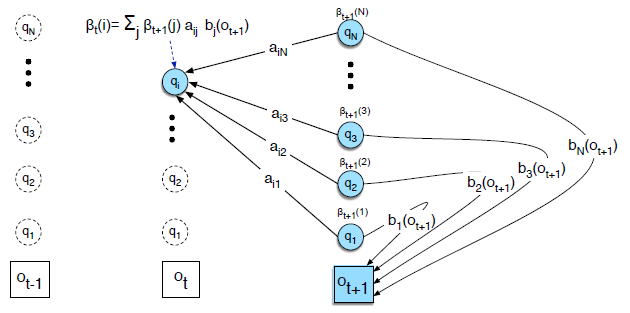
\includegraphics[scale=1]{viterbi/fig1 }
\end{center}
\caption{Viterbi trellis dùng cho việc tìm đường đi tốt nhất qua các không gian trạng thái ẩn cho việc ăn kem. Các trạng thái ẩn được đóng khung trong vòng tròn, các quan sát được đóng khung hình vuông. Các hình tròn nét đứt màu trắng thể hiện. Hình trên thể hiện quá trình tính $v_i \left( j \right)$ cho 2 trạng thái ở 2 bước. Quá trình tính toán trong mỗi ô sử dụng công thức (\ref{form2}) $v_t \left( j \right) = max_{1 \leqslant N - 1}v_{t - 1}a_{ij}b_j \left( {o_t} \right)$. Xác suất trong mỗi ô được tính theo công thức (\ref{form1}) $v_t \left( j \right) = P \left( {q_0, q_1, ..., q_{t - 1}, o_1, o_2, ..., o_t, q_t = \left. j \right|\lambda} \right).$ \label{viterbi_fig1}}
\end{figure}
Hình \ref{viterbi_fig1} cho ta một ví dụ về Viterbi trellis về tìm chuỗi trạng thái ẩn tốt nhất cho chuỗi quan sát $3 \text{ } 1 \text{ } 3.$ Ý tưởng là xử lý chuỗi quan sát từ trái sang phải, điền vào những trellis. Mỗi ô trong trellis, $v_t \left( j \right),$ thể hiện xác suất mô hình Markov ẩn ở trạng thái $j$ sau khi trải qua $t$ quan sát và đã duyệt qua các trạng thái có thể $q_1, q_2, ..., q_{t - 1},$ với tự động hóa $\lambda$ biết trước. Giá trị mỗi ô $v_t \left( j \right)$ được tính đệ quy bằng cách sử dụng đường đi có thể xảy ra nhất dẫn tới ô đó. Mỗi ô thể hiện xác suất được tính bằng công thức sau:
\begin{equation}
{v_t}\left( j \right) = \mathop {\max }\limits_{{q_1} \ldots {q_{t - 1}}} P\left( {\left. {{q_1} \ldots {q_{t - 1}},{o_1},{o_2} \ldots {o_t},{q_t} = j} \right|\lambda } \right).
\label{form1}
\end{equation}
Cần lưu ý rằng ta lấy đại diện con đường có thể xảy ra nhất bằng cách lấy giá trị lớn nhất của các chuỗi trạng thái trước đó $\mathop {\max }\limits_{{q_1} \ldots {q_{t - 1}}}.$ Giống như các thuật toán quy hoạch động khác, thuật toán Viterbi điền giá trị vào mỗi ô bằng phương pháp đệ quy. Biết rằng ta đã tính xác suất của mỗi trang thái ở thời điểm $t - 1,$ ta tính xác suất Viterbi bằng cách tìm mở rộng (extensions) có thể nhất của con đường dẫn đến ô hiện tại. VỚi mỗi trạng thái $q_j$ cho trước ở thời điểm $t,$ giá trị $v_t \left( j \right)$ được tính như sau:
\begin{equation}
{v_t}\left( j \right) = \mathop {\max }\limits_{i = 1}^N {v_{t - 1}}\left( i \right){a_{ij}}{b_j}\left( {{o_t}} \right).
\label{form2}
\end{equation}
3 nhân tử trong công thức (\ref{form2}) được sử dụng cho việc mở rộng con đường trước đó để tính xác suất Viterbi ở thời điểm $t:$
\begin{mybox}
$v_{t - 1} \left( i \right):$ xác suất con đường Viterbi (previous Viterbi path probability) từ bước trước đó.\\
$a_{ij}:$ xác suất chuyển (transition probability) từ trạng thái $q_i$ trước đó sang trạng thái $q_j$ hiện tại.\\
$b_j \left( {o_t} \right):$ độ hợp lý (state observation likelihood) của quan sát $o_t$ từ trạng thái $j.$
\end{mybox}
Mã giả của thuật toán Viterbi như sau:
\begin{breakablealgorithm}
  \caption{Thuật toán Viterbi}
  \begin{algorithmic}[1]
    \Function{Viterbi}{$observation \text{ of len } T, state\_graph \text{ of len } N$} 
   \State $\text{tạo một ma trân xác suất đường đi } viterbi[N, T]$
    \State \Comment{khởi tạo}
    \For {$\text{mỗi trạng thái } s$ \textbf{from} $1$ \textbf{to} $N$}
        \State $viterbi[s,1] \gets \pi_s * b_s \left( {o_1} \right)$
        \State $backpointer[s, 1] \gets 0$
        \State \Comment {đệ quy}
     \EndFor
     \For {$\text{mỗi bước}$ $t$ \textbf{from} $2$ \textbf{to} $T$}
        \For {$\text{mỗi trạng thái } s$ \textbf{from} $1$ \textbf{to} $N$}
        	\State $viterbi[s, t] \gets \mathop {\max }\limits_{s' = 1}^N \left( {viterbi\left[ {s',t - 1} \right]*{a_{s',s}}*{b_s}\left( {{o_t}} \right)} \right)$
        	\State $backpointer[s, t] \gets \mathop {\arg \max }\limits_{s' = 1}^N \left( {viterbi\left[ {s',t - 1} \right]*{a_{s',s}}*{b_s}\left( {{o_t}} \right)} \right)$
        \EndFor
      \EndFor
     \State \Comment{Kết thúc}
     \State $best\_path\_prob \gets \mathop {\max }\limits_{s = 1}^N \left( {viterbi\left[ {s,T} \right]} \right)$
     \State $best\_path\_pointer \gets \mathop {\arg \max }\limits_{s = 1}^N \left( {viterbi\left[ {s,T} \right]} \right) $
     \State $best\_path \gets \text{con đường bắt đầu ở trạng thái }  best\_path\_pointer, $
     \State $\text{, đi theo } backpointer[] \text{ đến các trạng thái}$
    \Return $best\_path, best\_path\_prob$
    \EndFunction
  \end{algorithmic}
\end{breakablealgorithm}

Thuật toán Viterbi tương tự như thuật toán tiến trước, ngoại trừ việc thuật toán này lấy \textbf{giá trị lớn nhất} của các xác suất đường đi (path probabilities) trước đó trong khi thuật toán tiến trước lấy \textbf{tổng}. Ngoài ra, thuật toán Viterbi có thêm một thành phần so với thuật toán tiến trước: \textbf{backpointer}. Lý do cho sự khác biệt này là trong khi thuật toán tiến trước cần cung cấp một độ hợp lý quan sát (observation likelihood), thuật toán Viterbi cần cung cấp xác suất và chuỗi trạng thái hợp lý nhất. Ta tính chuỗi trạng thái tốt nhất này bằng cách lưu lại vết (keep track) của đường đi từ các trạng thái ẩn dẫn tới mỗi trạng thái, giống như trong hình \ref{viterbi_fig2}, và sau đó, quay lại tìm đường đi tốt nhất tới trạng thái đầu (Viterbi backtrace).

\begin{figure}[H]
\begin{center}
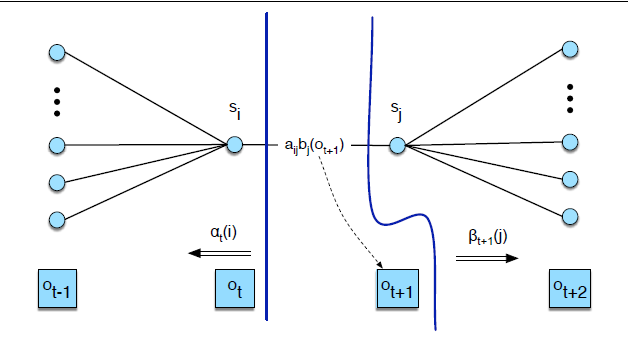
\includegraphics[scale=1]{viterbi/fig2}
\end{center}
\caption{Viterbi backtrace \label{viterbi_fig2}}
\end{figure}

Ta có định nghĩa của thuật toán Viterbi như sau:
\begin{enumerate}
\item Khởi tạo:
$${v_1}\left( j \right) = {\pi _j}{b_j}\begin{array}{*{20}{c}}
  {}&{1 \leqslant j \leqslant N} 
\end{array}$$
$$b{t_1}\left( j \right) = 0\begin{array}{*{20}{c}}
  {}&{1 \leqslant j \leqslant N} 
\end{array}$$
\item Đệ quy:
$${v_t}\left( j \right) = \mathop {\max }\limits_{i = 1}^N \left( {v{}_{t - 1}\left( i \right){a_{ij}}{b_j}\left( {{o_t}} \right)} \right)\begin{array}{*{20}{c}}
  {}&{1 \leqslant j \leqslant N,1 < t \leqslant T} 
\end{array}$$
$$b{t_t}\left( j \right) = \mathop {\max }\limits_{i = 1}^N \left( {v{}_{t - 1}\left( i \right){a_{ij}}{b_j}\left( {{o_t}} \right)} \right)\begin{array}{*{20}{c}}
  {}&{1 \leqslant j \leqslant N,1 < t \leqslant T} 
\end{array}$$
\item Kết thúc:\\
\begin{center}
Xác suất tốt nhất: $P* = \mathop {\max }\limits_{i = 1}^N \left( {{v_T}\left( i \right)} \right)$\\
Điểm bắt đầu của con đường tốt nhất: $q_T* = \mathop {\arg \max }\limits_{i = 1}^N \left( {{v_T}\left( i \right)} \right)$
\end{center}
\end{enumerate}